\documentclass[border=2pt]{standalone}
\usepackage{times}
\usepackage[T1]{fontenc}
\usepackage{tikz}
\usetikzlibrary{arrows.meta,positioning,fit,calc}
\begin{document}
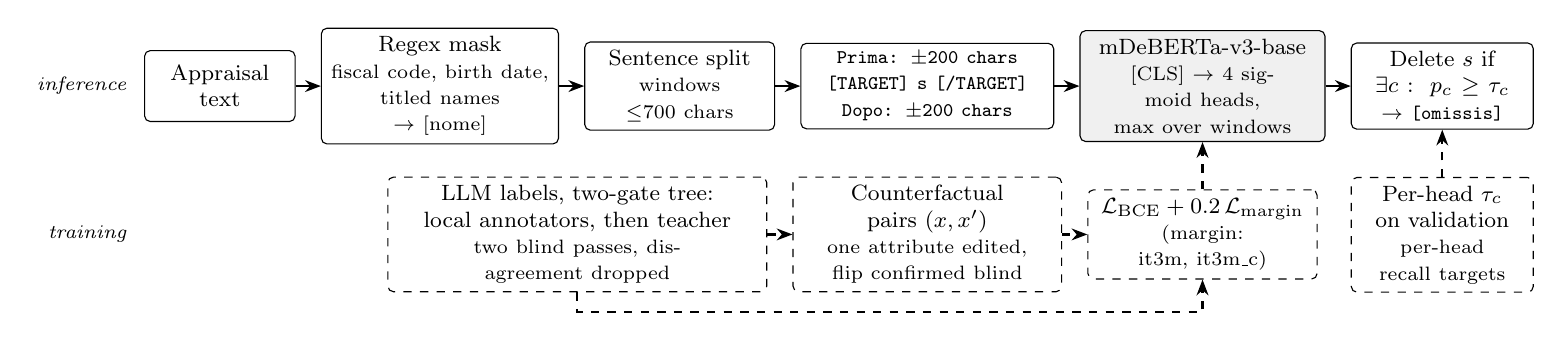
\begin{tikzpicture}[
  font=\footnotesize,
  box/.style={draw, rounded corners=2pt, align=center, inner sep=3pt, minimum height=9mm, text width=#1},
  box/.default=21mm,
  dbox/.style={draw, dashed, rounded corners=2pt, align=center, inner sep=3pt, minimum height=9mm, text width=#1},
  dbox/.default=21mm,
  arr/.style={-{Stealth[length=2mm]}, thick},
  node distance=4mm and 3.2mm
]
% inference row
\node[box=17mm] (doc) {Appraisal\\text};
\node[box=28mm, right=of doc] (mask) {Regex mask\\{\scriptsize fiscal code, birth date,}\\{\scriptsize titled names $\to$ [nome]}};
\node[box=22mm, right=of mask] (seg) {Sentence split\\{\scriptsize windows $\le$700 chars}};
\node[box=30mm, right=of seg] (fmt) {\texttt{\scriptsize Prima: $\pm$200 chars}\\\texttt{\scriptsize [TARGET] s [/TARGET]}\\\texttt{\scriptsize Dopo: $\pm$200 chars}};
\node[box=29mm, right=of fmt, fill=black!6] (enc) {mDeBERTa-v3-base\\{\scriptsize [CLS] $\to$ 4 sigmoid heads,}\\{\scriptsize max over windows}};
\node[box=21mm, right=of enc] (thr) {Delete $s$ if\\$\exists c:\ p_c \ge \tau_c$\\{\scriptsize $\to$ \texttt{[omissis]}}};
\draw[arr] (doc) -- (mask);
\draw[arr] (mask) -- (seg);
\draw[arr] (seg) -- (fmt);
\draw[arr] (fmt) -- (enc);
\draw[arr] (enc) -- (thr);
% training row
\node[dbox=27mm, below=6mm of enc] (loss) {$\mathcal{L}_{\mathrm{BCE}} + 0.2\,\mathcal{L}_{\mathrm{margin}}$\\{\scriptsize (margin: it3m, it3m\_c)}};
\node[dbox=21mm, below=6mm of thr] (val) {Per-head $\tau_c$\\on validation\\{\scriptsize per-head recall targets}};
\node[dbox=32mm, left=of loss] (pairs) {Counterfactual pairs $(x,x')$\\{\scriptsize one attribute edited,}\\{\scriptsize flip confirmed blind}};
\node[dbox=46mm, left=of pairs] (teach) {LLM labels, two-gate tree:\\local annotators, then teacher\\{\scriptsize two blind passes, disagreement dropped}};
\draw[arr, dashed] (teach) -- (pairs);
\draw[arr, dashed] (pairs) -- (loss);
\draw[arr, dashed] (loss) -- (enc);
\draw[arr, dashed] (teach.south) -- ++(0,-2.5mm) -| (loss.south);
\draw[arr, dashed] (val) -- (thr);
\node[anchor=east, font=\scriptsize\itshape] at ($(doc.west |- teach.west)+(-1mm,0)$) {training};
\node[anchor=east, font=\scriptsize\itshape] at ($(doc.west)+(-1mm,0)$) {inference};
\end{tikzpicture}
\end{document}
